\documentclass[conference]{IEEEtran}
\IEEEoverridecommandlockouts
% The preceding line is only needed to identify funding in the first footnote. If that is unneeded, please comment it out.
\usepackage{cite}
\usepackage{amsmath,amssymb,amsfonts}
\usepackage{algorithmic}
\usepackage{graphicx}
\usepackage{textcomp}
\usepackage{hyperref}
\usepackage{xcolor}
\def\BibTeX{{\rm B\kern-.05em{\sc i\kern-.025em b}\kern-.08em
    T\kern-.1667em\lower.7ex\hbox{E}\kern-.125emX}}
\begin{document}

\title{Humanoid Sprinting and Stopping DRL}

\author{

    \IEEEauthorblockN{Carlos Veríssimo}
    \IEEEauthorblockA{\textit{Department of Informatics Engineering} \\
        \textit{FEUP}\\
        Porto, Portugal \\
        up201907716@up.pt }
    \and

    \IEEEauthorblockN{Miguel Amorim}
    \IEEEauthorblockA{\textit{Department of Informatics Engineering } \\
        \textit{FEUP}\\
        Porto, Portugal \\
        up201907756@up.pt }
    \and

    \IEEEauthorblockN{Rafael Camelo}
    \IEEEauthorblockA{\textit{Department of Informatics Engineering } \\
        \textit{FEUP}\\
        Porto, Portugal \\
        up201907729@up.pt }
}


\maketitle

\begin{abstract}

\end{abstract}

\begin{IEEEkeywords}
    RoboCup, RoboCup 3D Simulation League, Reinforcement Learning, Humanoid Sprinting, Humanoid Stopping, Soccer
\end{IEEEkeywords}

\section{Introduction}

Reinforcement learning (RL) is a machine learning field in which agents learn optimal behaviours through trial-and-error interactions with their environment to maximize rewards and minimize punishments.

The RoboCup, which began in 1997, is a well-known platform for promoting robots and AI by pushing participants with tasks such as soccer, rescue, and home care. \cite{robocup97}.

This article digs into RoboCup's 3D Simulation League, introduced in 2004. The league evolved from using simple spheres to humanoid robots and now uses a simulated version of the NAO robot, a 58-cm-tall robot with 25 degrees of freedom (DOF) \cite{naorobot}, as the robot model.

\begin{figure}[htbp]
    \centerline{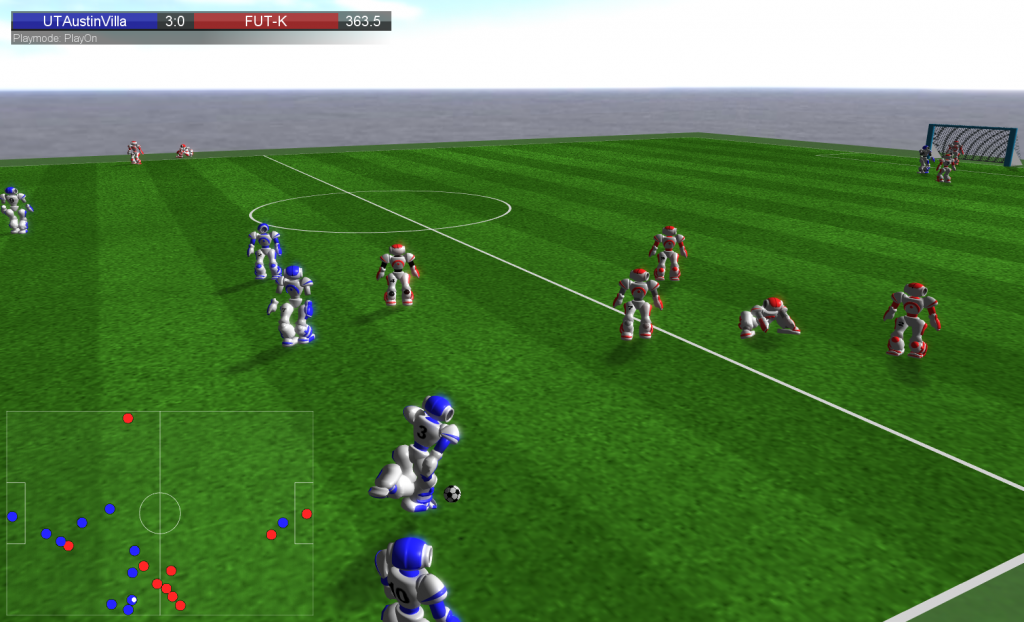
\includegraphics[width=0.35\textwidth]{images/robocup3d.png}}
    \caption{RoboCup 3D Simulation League.}
    \label{fig:robocup3d}
\end{figure}

To enforce physics laws, coordinate communications between the server and clients, and officiate the game, the league uses the SimSpark simulator.

Sprinting is an important feature of robotic soccer and plays a key role in team success. This paper also focuses on the difficult problem of stopping a run without falling, a feat that necessitates detailed control over the robot's numerous joints and sensors.

This study focuses on improving humanoid robot running and halting in the RoboCup 3D Simulation League.
Recognizing the intricacy and significance of these talents in robotic soccer, we intend to expand on previous advances in the field.
Our primary goal is to create solid, reliable techniques for accelerating and decelerating without falling by making use of comprehensive control
of the robot's joints and sensors.

We intend to build upon FC Portugual's efforts to improve humanoid robot running and stopping, and will use existing Gym environments to train our agent.
The FC Portugal's team repository can be found \href{https://github.com/m-abr/FCPCodebase}{https://github.com/m-abr/FCPCodebase}

This repository was created to ease the development of a team for the RoboCup 3D Simulation League.
It contains a set of tools and scripts that allow the user to train and test a team of simulated robots.

Subsequent sections detail related works (Section \ref{Related Work}), our methodology (Section \ref{Methodology}),
the significant results and their implications (Section \ref{Results and Discussion}),
concluding with future directions for this field (Section \ref{Conclusions and Future Work})

\section{Related Work}\label{Related Work}

Yearly held in different countries, the RoboCup, and, in particular, its 3D Simulated Soccer League, has been a platform for the development of new techniques and algorithms in the field of robotics and artificial intelligence.
Teams that wish to participate in the league must submit a Team Description Paper (TDP) that describes their team's research and development efforts in the previous years.

Papers from FC Portugal were studied to understand the state of the art in the field of humanoid sprinting and stopping.

In 2020, FC Portugal's TDP \cite{lau2020fc} introduced two new skills: running and sprinting. These skills were learned using
a Proximal Policy Optimization (PPO) reinforcement learning algorithm.

All joints but the head were used to control the robot's movements and angles are controlled using a proportional controller.

The sprinting skill is less focused on turning and more on running in a straight line and ends in one of three ways:
the robot kicks the ball, the robot transitions into walking, or the robot stops.

When running, the outcomes are the same as when sprinting, except that the robot does kick the ball.

A paper by Abreu et al. \cite{10.1007/978-3-030-35699-6_1} describes the team's efforts to leverage the Proximo Policy Optimization (PPO)
algorithm using information provided by the simulator to learn how to run faster, in a stable manner, and stopping.

The reseachers used an implementation of the PPO algorithm provided by OpenAI's Baselines library, which involved
clipped surrogate objective and alternating between data sampling and stochastic gradient ascent. The authors adapted hyperparameters from OpenAI's work with a
3D humanoid model in mujoco, making adjustments for their specific tasks.

In regards to the experimental setup and testing, the setups were the same for the spriting behaviour: the robot is placed near the left goal, facing the other
goal.

The robot's objective is to run as fast as possible, in a straight line, and the reward is based on it's torso's x-coordinate difference
from the last step. The more the robot runs, the higher the reward.

The stopping behaviour was only trained after optimizing the running behaviour.
The robot is placed in the same initial pose as before, and runs for some time until the stopping behaviour is triggered.

The reseachers managed to stabalize the robot's sprinting behaviour, at around 2.5 m/s.

\section{Methodology}\label{Methodology}

In this section, we outline the key components of our simulator and the agent used for training and testing.
The primary objective is to design an environment for training a humanoid agent that can both sprint and stop without falling.


\subsection{Simulator and Agent}\label{Simulator and Agent}

As mentioned before, we intend on using the FC Portugal's team repository as a basis for our work.

An integration with OpenAI gym is provided, which allows us to use the gym environment to train, test and evaluate our agent.

Simspark is used as the simulator, which is a 3D simulator for humanoid robots. It serves as the underlying physics engine that replicates the physical world in which our agent operates.
It allows us to model sprinting and stopping behaviors realistically, providing a high-fidelity simulation environment.

The agent used is a simulated representation of the NAO robot.

\subsection{State Space}\label{State Space}

The state space represents the information available to the agent at each time step. It includes various sensory inputs and internal variables that capture the robot's state within the SimSpark environment.
Our state space is composed by 70 variables, describing the robot's position, orientation, velocities, accelerations, and angles of all joints.

Figure \ref{fig:nao-joints} shows the robot's joints.

\begin{figure}[htbp]
    \centerline{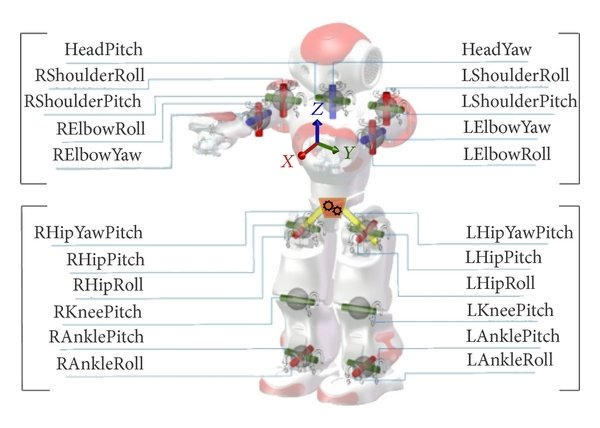
\includegraphics[width=0.35\textwidth]{images/joints.png}}
    \caption{Nao's joints.}
    \label{fig:nao-joints}
\end{figure}

\subsection{Action Space}\label{Action Space}

The action space defines the set of actions that the agent can take to interact with the SimSpark environment. Our action space comprises 22 continuous
dimensions, each corresponding to a specific joint or motion parameter. These actions allow the agent to control its movements and execute complex motor actions within the simulator.

\subsection{Reward Function}\label{Reward Function}

The reward function is structured to assess various aspects of the robot's walking behavior, each contributing to a cumulative score that reflects the efficacy and naturalness of its movements.

The reward function is composed of 7 components, each with a different weight, which are summed to obtain the final reward:
\begin{itemize}
    \item \textbf{Arm Coordination and Movement}: The function evaluates the coordination between the robot's arms, rewarding movements where the arms swing in opposite directions,
          reminiscent of human walking. This aspect encourages not only coordination but also ensures that arm movements contribute positively to the overall balance and momentum.
    \item \textbf{Leg Coordination}: Similar to arm coordination, leg movements are rewarded based on their coordinated and alternating action. This evaluation is crucial for a bipedal gait, as it promotes a stable and efficient step cycle.
    \item \textbf{Opposite Arm and Leg Coordination}: Emulating the natural human gait, the reward function encourages the opposite movement of arms and legs. This coordination is vital for maintaining balance and forward momentum.
    \item \textbf{Posture and Elevation Penalties}: To discourage a posture that might lead to instability or falls, the robot is penalized for low torso and head heights. Maintaining an upright position is fundamental for effective bipedal locomotion.
    \item \textbf{Head Stability}: Stability in the robot's head movement is rewarded, as excessive oscillation can disrupt balance and visual processing, which are essential for navigating complex environments.
    \item \textbf{Joint Movement Reward}: Movement in the robot's joints, particularly in the limbs, contributes positively to the reward. This aspect ensures that the robot does not remain static and encourages dynamic movement essential for walking.
    \item \textbf{Forward Movement Incentive}: One of the primary goals of the reward function is to promote forward movement. The robot earns rewards for advancing forward, whereas moving backward incurs penalties. This aspect is crucial for achieving the primary objective of walking.
    \item \textbf{Torso Orientation}: An upright or slightly forward-leaning torso orientation is rewarded. This posture is typical in human walking and helps in maintaining balance and forward momentum.
\end{itemize}

\subsection{Optimization Algorithm}\label{Optimization Algorithm}




\section{Results and Discussion}\label{Results and Discussion}

\section{Conclusions and Future Work}\label{Conclusions and Future Work}

\section{Acknowledgments}\label{Acknowledgments}

First and foremost, we would like to express our gratitude for the collaboration and cooperation we have maintained throughout this relatively brief yet intricate task.

Secondly, we thank the course's professors, for their guidance and support throughout the development
of this project.

Finally, we would also like to extend our gratitude to the members involved in the development of the FC Portugal's team repository, for their work and for making it available to the public.

\begin{thebibliography}{00}
    \bibitem{lau2020fc}Lau, N., Reis, L., Simoes, D., Abreu, M., Silva, T. \& Resende, F. FC Portugal 3D Simulation Team: Team Description Paper 2020.  (2023)
    \bibitem{10.1007/978-3-030-35699-6_1}Abreu, M., Reis, L. \& Lau, N. Learning to Run Faster in a Humanoid Robot Soccer Environment Through Reinforcement Learning. {\em RoboCup 2019: Robot World Cup XXIII}. pp. 3-15 (2019)
    \bibitem{naorobot} Nao the Humanoid and Programmable Robot, \href{www.aldebaran.com/en/nao}{www.aldebaran.com/en/nao}. Last accessed 24 Dec 2023
    \bibitem{robocup97} Noda, I., Suzuki, S. J., Matsubara, H., Asada, M., Kitano, H.: RoboCup-97: The first robot world cup soccer games and conferences. AI magazine 19(3), 49-49 (1998)
\end{thebibliography}

\end{document}
